Die Framework Anwendung soll nur OCPP-Schnittstelle benutzen. 
Die HTTP- und Filesystem- Schnittstelle werden gar nicht gebraucht und deswegen müssen gemockt werden.
Die Datenbank-Schnittstelle soll gefälscht werden, da es gewünscht wird, 
manche Informationen zu speichern um sie später verwenden bzw. auswerten zu können.

Die Anwendung lässt sich wie folgt darstellen 
(Die blaue Farbe stellt gefälschte Komponenten dar, die schwarze Farbe stellt gefälschte Komponente dar):

\import{./images/solutions}{Framework}

\newpage
Das Framework wird von den Dritten benutzt. Aus diesen Grund benötigt es ein gutes Interfaces, 
das zugleich als Fassade (siehe Kapitel \ref{kap:gof:facade}) zu der Struktur in der Abbildung \ref{fig:solutionFramework} darstellt.

Die Struktur als Klassendiagramm:
\textbf{HIER SOLL DIE Struktrur des FRAMEWORKS SEIN}

Das Interface besteht aus folgende Methoden:
\begin{itemize}
    \item start
    \item stop
    \item addUseCase
    \item rewriteUseCase
    \item waitOf
    \item waitOfNextEvent
    \item sendMessage
\end{itemize}

Jeder Test lässt sich in vier Phasen unterteilen, jede Methode bzw. Funktion des Frameworks soll einer dieser Phase zugeordnet werden.
In der nachfolgenden Abbildung \ref{fig:TestFlow} ist eine Zuordnung der Methoden zu jeweiliger Phase im From eines Ablaufdiagramms zu sehen:

\begin{figure}[H]
    \centering
    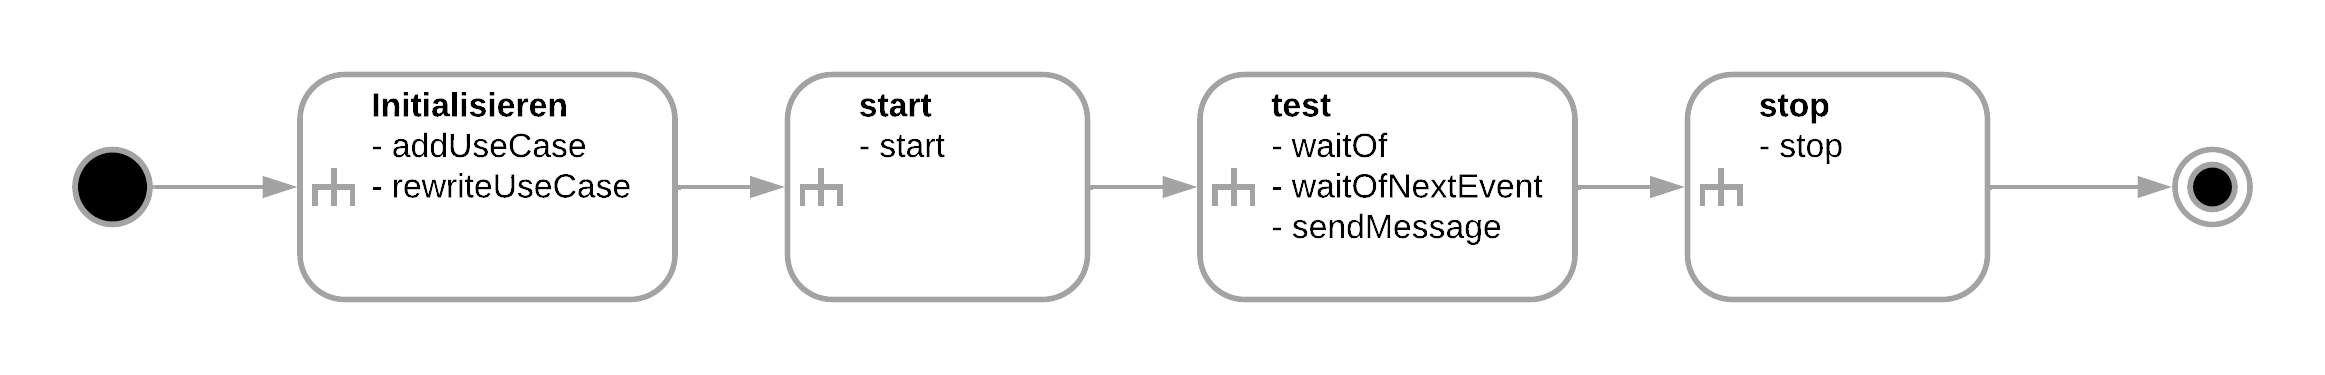
\includegraphics[width=1\textwidth]{./images/TestAblauf.png}
    \caption[Ablaufdiagramm eines Tests]{Ablaufdiagramm eines Tests}
    \label{fig:TestFlow}
\end{figure}